\PassOptionsToPackage{unicode=true}{hyperref} % options for packages loaded elsewhere
\PassOptionsToPackage{hyphens}{url}
%
\documentclass[]{article}
\usepackage{lmodern}
\usepackage{amssymb,amsmath}
\usepackage{ifxetex,ifluatex}
\usepackage{fixltx2e} % provides \textsubscript
\ifnum 0\ifxetex 1\fi\ifluatex 1\fi=0 % if pdftex
  \usepackage[T1]{fontenc}
  \usepackage[utf8]{inputenc}
  \usepackage{textcomp} % provides euro and other symbols
\else % if luatex or xelatex
  \usepackage{unicode-math}
  \defaultfontfeatures{Ligatures=TeX,Scale=MatchLowercase}
\fi
% use upquote if available, for straight quotes in verbatim environments
\IfFileExists{upquote.sty}{\usepackage{upquote}}{}
% use microtype if available
\IfFileExists{microtype.sty}{%
\usepackage[]{microtype}
\UseMicrotypeSet[protrusion]{basicmath} % disable protrusion for tt fonts
}{}
\IfFileExists{parskip.sty}{%
\usepackage{parskip}
}{% else
\setlength{\parindent}{0pt}
\setlength{\parskip}{6pt plus 2pt minus 1pt}
}
\usepackage{hyperref}
\hypersetup{
            pdftitle={Milestone 03 - Group 09},
            pdfauthor={Daniel Hadley, Kristina Wright},
            pdfborder={0 0 0},
            breaklinks=true}
\urlstyle{same}  % don't use monospace font for urls
\usepackage[margin=1in]{geometry}
\usepackage{color}
\usepackage{fancyvrb}
\newcommand{\VerbBar}{|}
\newcommand{\VERB}{\Verb[commandchars=\\\{\}]}
\DefineVerbatimEnvironment{Highlighting}{Verbatim}{commandchars=\\\{\}}
% Add ',fontsize=\small' for more characters per line
\usepackage{framed}
\definecolor{shadecolor}{RGB}{248,248,248}
\newenvironment{Shaded}{\begin{snugshade}}{\end{snugshade}}
\newcommand{\AlertTok}[1]{\textcolor[rgb]{0.94,0.16,0.16}{#1}}
\newcommand{\AnnotationTok}[1]{\textcolor[rgb]{0.56,0.35,0.01}{\textbf{\textit{#1}}}}
\newcommand{\AttributeTok}[1]{\textcolor[rgb]{0.77,0.63,0.00}{#1}}
\newcommand{\BaseNTok}[1]{\textcolor[rgb]{0.00,0.00,0.81}{#1}}
\newcommand{\BuiltInTok}[1]{#1}
\newcommand{\CharTok}[1]{\textcolor[rgb]{0.31,0.60,0.02}{#1}}
\newcommand{\CommentTok}[1]{\textcolor[rgb]{0.56,0.35,0.01}{\textit{#1}}}
\newcommand{\CommentVarTok}[1]{\textcolor[rgb]{0.56,0.35,0.01}{\textbf{\textit{#1}}}}
\newcommand{\ConstantTok}[1]{\textcolor[rgb]{0.00,0.00,0.00}{#1}}
\newcommand{\ControlFlowTok}[1]{\textcolor[rgb]{0.13,0.29,0.53}{\textbf{#1}}}
\newcommand{\DataTypeTok}[1]{\textcolor[rgb]{0.13,0.29,0.53}{#1}}
\newcommand{\DecValTok}[1]{\textcolor[rgb]{0.00,0.00,0.81}{#1}}
\newcommand{\DocumentationTok}[1]{\textcolor[rgb]{0.56,0.35,0.01}{\textbf{\textit{#1}}}}
\newcommand{\ErrorTok}[1]{\textcolor[rgb]{0.64,0.00,0.00}{\textbf{#1}}}
\newcommand{\ExtensionTok}[1]{#1}
\newcommand{\FloatTok}[1]{\textcolor[rgb]{0.00,0.00,0.81}{#1}}
\newcommand{\FunctionTok}[1]{\textcolor[rgb]{0.00,0.00,0.00}{#1}}
\newcommand{\ImportTok}[1]{#1}
\newcommand{\InformationTok}[1]{\textcolor[rgb]{0.56,0.35,0.01}{\textbf{\textit{#1}}}}
\newcommand{\KeywordTok}[1]{\textcolor[rgb]{0.13,0.29,0.53}{\textbf{#1}}}
\newcommand{\NormalTok}[1]{#1}
\newcommand{\OperatorTok}[1]{\textcolor[rgb]{0.81,0.36,0.00}{\textbf{#1}}}
\newcommand{\OtherTok}[1]{\textcolor[rgb]{0.56,0.35,0.01}{#1}}
\newcommand{\PreprocessorTok}[1]{\textcolor[rgb]{0.56,0.35,0.01}{\textit{#1}}}
\newcommand{\RegionMarkerTok}[1]{#1}
\newcommand{\SpecialCharTok}[1]{\textcolor[rgb]{0.00,0.00,0.00}{#1}}
\newcommand{\SpecialStringTok}[1]{\textcolor[rgb]{0.31,0.60,0.02}{#1}}
\newcommand{\StringTok}[1]{\textcolor[rgb]{0.31,0.60,0.02}{#1}}
\newcommand{\VariableTok}[1]{\textcolor[rgb]{0.00,0.00,0.00}{#1}}
\newcommand{\VerbatimStringTok}[1]{\textcolor[rgb]{0.31,0.60,0.02}{#1}}
\newcommand{\WarningTok}[1]{\textcolor[rgb]{0.56,0.35,0.01}{\textbf{\textit{#1}}}}
\usepackage{longtable,booktabs}
% Fix footnotes in tables (requires footnote package)
\IfFileExists{footnote.sty}{\usepackage{footnote}\makesavenoteenv{longtable}}{}
\usepackage{graphicx,grffile}
\makeatletter
\def\maxwidth{\ifdim\Gin@nat@width>\linewidth\linewidth\else\Gin@nat@width\fi}
\def\maxheight{\ifdim\Gin@nat@height>\textheight\textheight\else\Gin@nat@height\fi}
\makeatother
% Scale images if necessary, so that they will not overflow the page
% margins by default, and it is still possible to overwrite the defaults
% using explicit options in \includegraphics[width, height, ...]{}
\setkeys{Gin}{width=\maxwidth,height=\maxheight,keepaspectratio}
\setlength{\emergencystretch}{3em}  % prevent overfull lines
\providecommand{\tightlist}{%
  \setlength{\itemsep}{0pt}\setlength{\parskip}{0pt}}
\setcounter{secnumdepth}{0}
% Redefines (sub)paragraphs to behave more like sections
\ifx\paragraph\undefined\else
\let\oldparagraph\paragraph
\renewcommand{\paragraph}[1]{\oldparagraph{#1}\mbox{}}
\fi
\ifx\subparagraph\undefined\else
\let\oldsubparagraph\subparagraph
\renewcommand{\subparagraph}[1]{\oldsubparagraph{#1}\mbox{}}
\fi

% set default figure placement to htbp
\makeatletter
\def\fps@figure{htbp}
\makeatother


\title{Milestone 03 - Group 09}
\author{Daniel Hadley, Kristina Wright}
\date{March 14, 2020}

\begin{document}
\maketitle

\hypertarget{airbnb-listings-for-barcelona}{%
\subsection{Airbnb Listings for
Barcelona}\label{airbnb-listings-for-barcelona}}

\hypertarget{introduction}{%
\subsubsection{Introduction}\label{introduction}}

Airbnb, Inc.~is a company founded in 2008 that offers an online
marketplace connecting people who offer lodging with people who require
accomodations in that locale. The company does not own any of the listed
properties and operates as a broker, collecting commissions once a
lodging is booked. As a direct competitor to hotels, we are interested
in how the users listing properties determine the price they charge.

When accomodations are offered through Airbnb, the person listing the
property is called a host, and they must provide a variety of
information about the listing including price, neighborhood, type of
accommodations offered, and the minimum number of nights a guest must
stay if they want to make a booking. In addition to information provided
by the host, Airbnb collects and disseminates information about the
listing which we use to perform our analysis.

The data is collected using public information compiled from the Airbnb
website. Specific collection techniques are not specified, though the
Inside Airbnb \href{http://insideairbnb.com/behind.html}{website} states
that it uses Open Source technologies such as D3, Boostrap, jQuery, etc.
to collect the data and much code was ``copied and pasted'' from the
internet. A major contributer to this code,
\href{http://tomslee.net/category/airbnb-data}{Tom Slee}, described it
as a ``scrape'' of the Airbnb website for each city.

\hypertarget{data-description}{%
\subsubsection{Data Description}\label{data-description}}

The \href{http://insideairbnb.com/get-the-data.html}{dataset} used in
this analysis is collected and offered by Inside Airbnb, an independent,
non-commercial project started by Murray Cox and John Morris. Their goal
is to allow people to see how Airbnb might be affecting the residential
housing market. We use the summary data for listings, since it includes
the data we are interested in exploring and is more manageable,
size-wise, than the detailed listings data.

The data used in this analysis was compiled on November 9, 2019 and
includes 20,428 Airbnb listings that travellers see when using the
Airbnb website to find accommodations in Barcelona, Spain. The table
below describes the available data for each listing in the dataset.

\begin{longtable}[]{@{}llll@{}}
\toprule
\begin{minipage}[b]{0.22\columnwidth}\raggedright
Variable Name\strut
\end{minipage} & \begin{minipage}[b]{0.22\columnwidth}\raggedright
Column Name\strut
\end{minipage} & \begin{minipage}[b]{0.22\columnwidth}\raggedright
Type of Data\strut
\end{minipage} & \begin{minipage}[b]{0.22\columnwidth}\raggedright
Description\strut
\end{minipage}\tabularnewline
\midrule
\endhead
\begin{minipage}[t]{0.22\columnwidth}\raggedright
Listing ID\strut
\end{minipage} & \begin{minipage}[t]{0.22\columnwidth}\raggedright
\texttt{id}\strut
\end{minipage} & \begin{minipage}[t]{0.22\columnwidth}\raggedright
Categorical/Numeric\strut
\end{minipage} & \begin{minipage}[t]{0.22\columnwidth}\raggedright
Numeric identifier unique to each listing\strut
\end{minipage}\tabularnewline
\begin{minipage}[t]{0.22\columnwidth}\raggedright
Name\strut
\end{minipage} & \begin{minipage}[t]{0.22\columnwidth}\raggedright
\texttt{name}\strut
\end{minipage} & \begin{minipage}[t]{0.22\columnwidth}\raggedright
Character\strut
\end{minipage} & \begin{minipage}[t]{0.22\columnwidth}\raggedright
Short title for the listing provided by the host\strut
\end{minipage}\tabularnewline
\begin{minipage}[t]{0.22\columnwidth}\raggedright
Host ID\strut
\end{minipage} & \begin{minipage}[t]{0.22\columnwidth}\raggedright
\texttt{host\_id}\strut
\end{minipage} & \begin{minipage}[t]{0.22\columnwidth}\raggedright
Categorical/Numeric\strut
\end{minipage} & \begin{minipage}[t]{0.22\columnwidth}\raggedright
Numeric identifier for the host of the listing\strut
\end{minipage}\tabularnewline
\begin{minipage}[t]{0.22\columnwidth}\raggedright
Host Name\strut
\end{minipage} & \begin{minipage}[t]{0.22\columnwidth}\raggedright
\texttt{host\_name}\strut
\end{minipage} & \begin{minipage}[t]{0.22\columnwidth}\raggedright
Categorical/String\strut
\end{minipage} & \begin{minipage}[t]{0.22\columnwidth}\raggedright
Name of the host or hosts of the listing provided by the host(s) to
Airbnb\strut
\end{minipage}\tabularnewline
\begin{minipage}[t]{0.22\columnwidth}\raggedright
Neighbourhood Group\strut
\end{minipage} & \begin{minipage}[t]{0.22\columnwidth}\raggedright
\texttt{neighbourhood\_group}\strut
\end{minipage} & \begin{minipage}[t]{0.22\columnwidth}\raggedright
Categorical/String\strut
\end{minipage} & \begin{minipage}[t]{0.22\columnwidth}\raggedright
Districts of Barcelona as determined by the coordinates of the listing
and the city's definition of its districts; this data is not the data
provided by the host\strut
\end{minipage}\tabularnewline
\begin{minipage}[t]{0.22\columnwidth}\raggedright
Neighbourhood\strut
\end{minipage} & \begin{minipage}[t]{0.22\columnwidth}\raggedright
\texttt{neighbourhood}\strut
\end{minipage} & \begin{minipage}[t]{0.22\columnwidth}\raggedright
Categorical/String\strut
\end{minipage} & \begin{minipage}[t]{0.22\columnwidth}\raggedright
Neighbourhoods of Barcelona are smaller geographical areas than
districts and are determined by the coordinates of the listing and
compared to the city's boundaries of its neighbourhoods; this data is
not the neighbourhood provided by the host\strut
\end{minipage}\tabularnewline
\begin{minipage}[t]{0.22\columnwidth}\raggedright
Latitude\strut
\end{minipage} & \begin{minipage}[t]{0.22\columnwidth}\raggedright
\texttt{latitude}\strut
\end{minipage} & \begin{minipage}[t]{0.22\columnwidth}\raggedright
Numeric\strut
\end{minipage} & \begin{minipage}[t]{0.22\columnwidth}\raggedright
Latitude coordinates of the listing\strut
\end{minipage}\tabularnewline
\begin{minipage}[t]{0.22\columnwidth}\raggedright
Longitude\strut
\end{minipage} & \begin{minipage}[t]{0.22\columnwidth}\raggedright
\texttt{longitude}\strut
\end{minipage} & \begin{minipage}[t]{0.22\columnwidth}\raggedright
Numeric\strut
\end{minipage} & \begin{minipage}[t]{0.22\columnwidth}\raggedright
Longitude coordinates of the listing\strut
\end{minipage}\tabularnewline
\begin{minipage}[t]{0.22\columnwidth}\raggedright
Type of Accommodation\strut
\end{minipage} & \begin{minipage}[t]{0.22\columnwidth}\raggedright
\texttt{room\_type}\strut
\end{minipage} & \begin{minipage}[t]{0.22\columnwidth}\raggedright
Categorical/String\strut
\end{minipage} & \begin{minipage}[t]{0.22\columnwidth}\raggedright
Type of accommodations specify whether the listing is for an entire home
or apartment, a private room in a shared home or apartment, a hotel
room, or a shared room\strut
\end{minipage}\tabularnewline
\begin{minipage}[t]{0.22\columnwidth}\raggedright
Price\strut
\end{minipage} & \begin{minipage}[t]{0.22\columnwidth}\raggedright
\texttt{price}\strut
\end{minipage} & \begin{minipage}[t]{0.22\columnwidth}\raggedright
Numeric\strut
\end{minipage} & \begin{minipage}[t]{0.22\columnwidth}\raggedright
The price per night, in euros, to book a listing\strut
\end{minipage}\tabularnewline
\begin{minipage}[t]{0.22\columnwidth}\raggedright
Minimum Stay\strut
\end{minipage} & \begin{minipage}[t]{0.22\columnwidth}\raggedright
\texttt{minimum\_nights}\strut
\end{minipage} & \begin{minipage}[t]{0.22\columnwidth}\raggedright
Numeric\strut
\end{minipage} & \begin{minipage}[t]{0.22\columnwidth}\raggedright
The minimum number of nights that a guest must reserve in order to book
a listing\strut
\end{minipage}\tabularnewline
\begin{minipage}[t]{0.22\columnwidth}\raggedright
Number of Reviews\strut
\end{minipage} & \begin{minipage}[t]{0.22\columnwidth}\raggedright
\texttt{number\_of\_reviews}\strut
\end{minipage} & \begin{minipage}[t]{0.22\columnwidth}\raggedright
Numeric\strut
\end{minipage} & \begin{minipage}[t]{0.22\columnwidth}\raggedright
The number of reviews left by guests after their stay\strut
\end{minipage}\tabularnewline
\begin{minipage}[t]{0.22\columnwidth}\raggedright
Last Review\strut
\end{minipage} & \begin{minipage}[t]{0.22\columnwidth}\raggedright
\texttt{last\_review}\strut
\end{minipage} & \begin{minipage}[t]{0.22\columnwidth}\raggedright
Date\strut
\end{minipage} & \begin{minipage}[t]{0.22\columnwidth}\raggedright
The date of the last review left by a guest\strut
\end{minipage}\tabularnewline
\begin{minipage}[t]{0.22\columnwidth}\raggedright
Reviews per Month\strut
\end{minipage} & \begin{minipage}[t]{0.22\columnwidth}\raggedright
\texttt{reviews\_per\_month}\strut
\end{minipage} & \begin{minipage}[t]{0.22\columnwidth}\raggedright
Numeric\strut
\end{minipage} & \begin{minipage}[t]{0.22\columnwidth}\raggedright
The number of reviews left by guests of a listing divided by the number
of months the listing has been active\strut
\end{minipage}\tabularnewline
\begin{minipage}[t]{0.22\columnwidth}\raggedright
Number of Listings by Host\strut
\end{minipage} & \begin{minipage}[t]{0.22\columnwidth}\raggedright
\texttt{calculated\_host\_listings\_count}\strut
\end{minipage} & \begin{minipage}[t]{0.22\columnwidth}\raggedright
Numeric\strut
\end{minipage} & \begin{minipage}[t]{0.22\columnwidth}\raggedright
A count of the number of listings under the same Host Name\strut
\end{minipage}\tabularnewline
\begin{minipage}[t]{0.22\columnwidth}\raggedright
Availability\strut
\end{minipage} & \begin{minipage}[t]{0.22\columnwidth}\raggedright
\texttt{availability\_365}\strut
\end{minipage} & \begin{minipage}[t]{0.22\columnwidth}\raggedright
Numeric\strut
\end{minipage} & \begin{minipage}[t]{0.22\columnwidth}\raggedright
The number of days over the next 365 days that the listing can be booked
by guests; calculated as 365 minus booked days minus days listing is
unavailable as per the host\strut
\end{minipage}\tabularnewline
\bottomrule
\end{longtable}

\hypertarget{exploring-the-dataset}{%
\subsubsection{Exploring the Dataset}\label{exploring-the-dataset}}

\hypertarget{remove-unwanted-data}{%
\paragraph{Remove Unwanted Data}\label{remove-unwanted-data}}

In this section, we remove columns from the dataset that should have no
fundamental influence on listing price. This includes the short title of
the listing (\texttt{name}), the name of the host(s)
(\texttt{host\_name}), and the availability of the listing over the next
365 days (\texttt{availability\_365}). While there might end up being a
relation between availability and price, since cheap listings for a
desirable neighbourhood are likely to be booked, this relationship is
backwards; we want to find factors that affect the listing price, not
factors affected by the listing price.

\hypertarget{rename-columns}{%
\paragraph{Rename Columns}\label{rename-columns}}

Some of the column names are a little long, so we perform the following
renamings:

\begin{itemize}
\item
  \texttt{neighbourhood\_group} is renamed to \texttt{district}
\item
  \texttt{minimum\_nights} is renamed to \texttt{min\_stay}
\item
  \texttt{number\_of\_reviews} is renamed to \texttt{reviews}
\item
  \texttt{calculated\_host\_listings\_count} is renamed to
  \texttt{host\_listings}
\end{itemize}

\hypertarget{filter-data}{%
\paragraph{Filter Data}\label{filter-data}}

A few extreme outliers skew the density of the price of listings to the
right. As a result, we exclude the top 2.5\% of listings. Then, we
exclude listings with a minimum stay over 5 nights. This should help to
limit listings that are catered to tourists by eliminating listings that
are better classified as short-term rentals.

\hypertarget{price-density}{%
\paragraph{Price Density}\label{price-density}}

A kernel density plot is presented for listing prices. An interesting
observation from the price density is the tendency for people to price
their listings in increments of 50 Euros. For example, the Density Plot,
we see multi-modes, where each mode after the largest mode occurs at
every 50 Euro increment along the x-axis

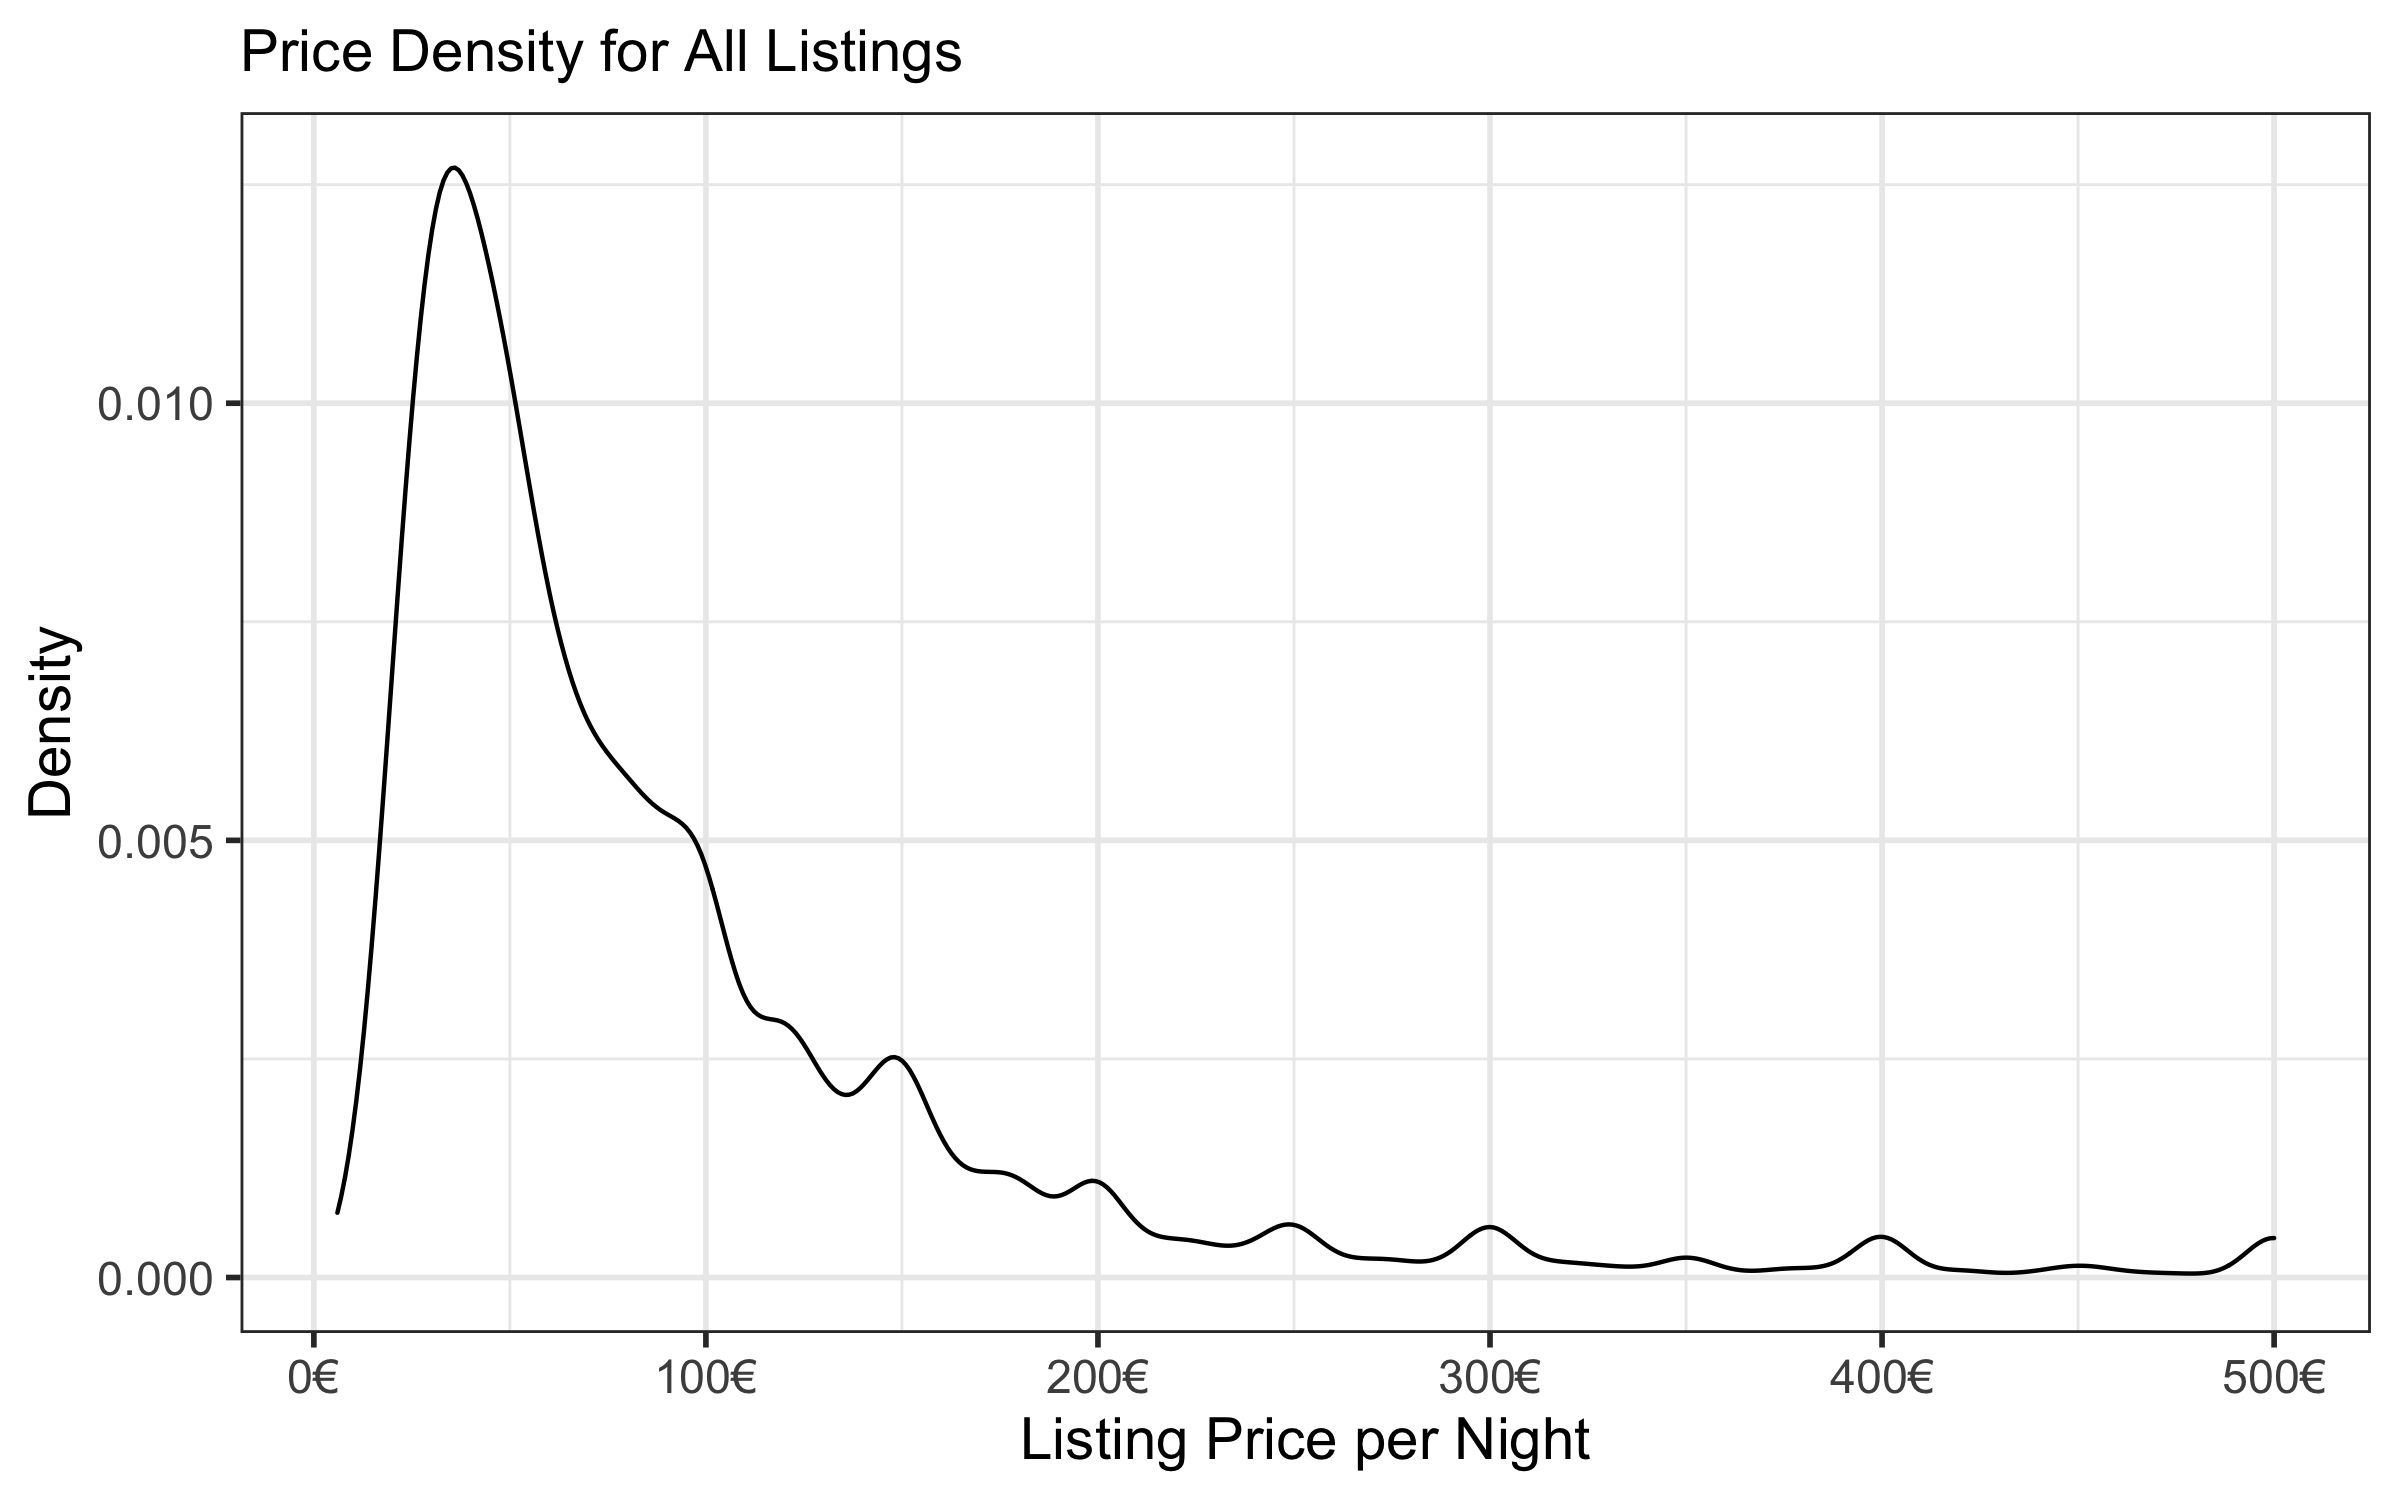
\includegraphics[width=6.77083in,height=\textheight]{../images/density_plot.png}

\hypertarget{correlogram}{%
\paragraph{Correlogram}\label{correlogram}}

Based on the correlogram shown below there is little correlation between
the 6 numerical variables presented. All positive correlations are in
blue, and all negative correlations are in red.

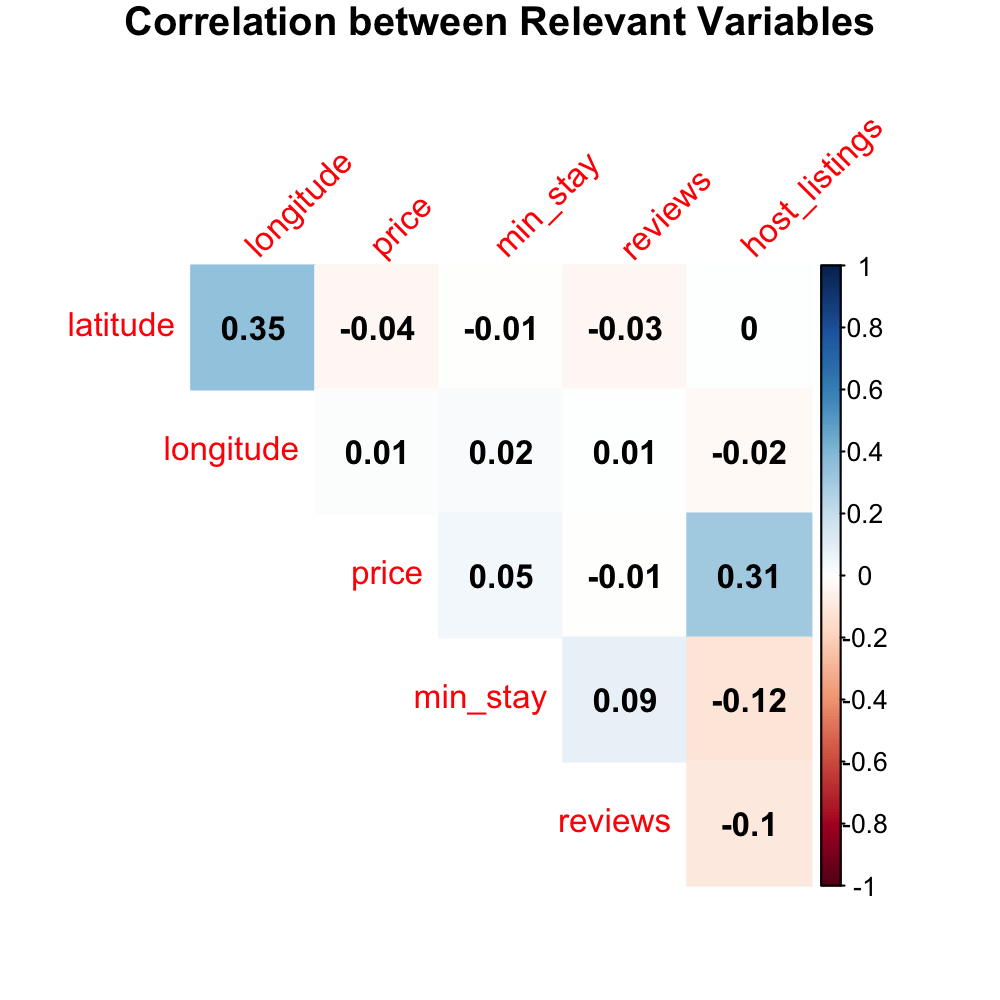
\includegraphics[width=5.20833in,height=\textheight]{../images/correlogram.png}

\hypertarget{violin-plot}{%
\paragraph{Violin Plot}\label{violin-plot}}

The violin plot below shows the distribution of price in log10 scale for
each district in descending order of average price. Based on the plot,
Example has the highest priced and Nou Barris has the lowest priced
listings.

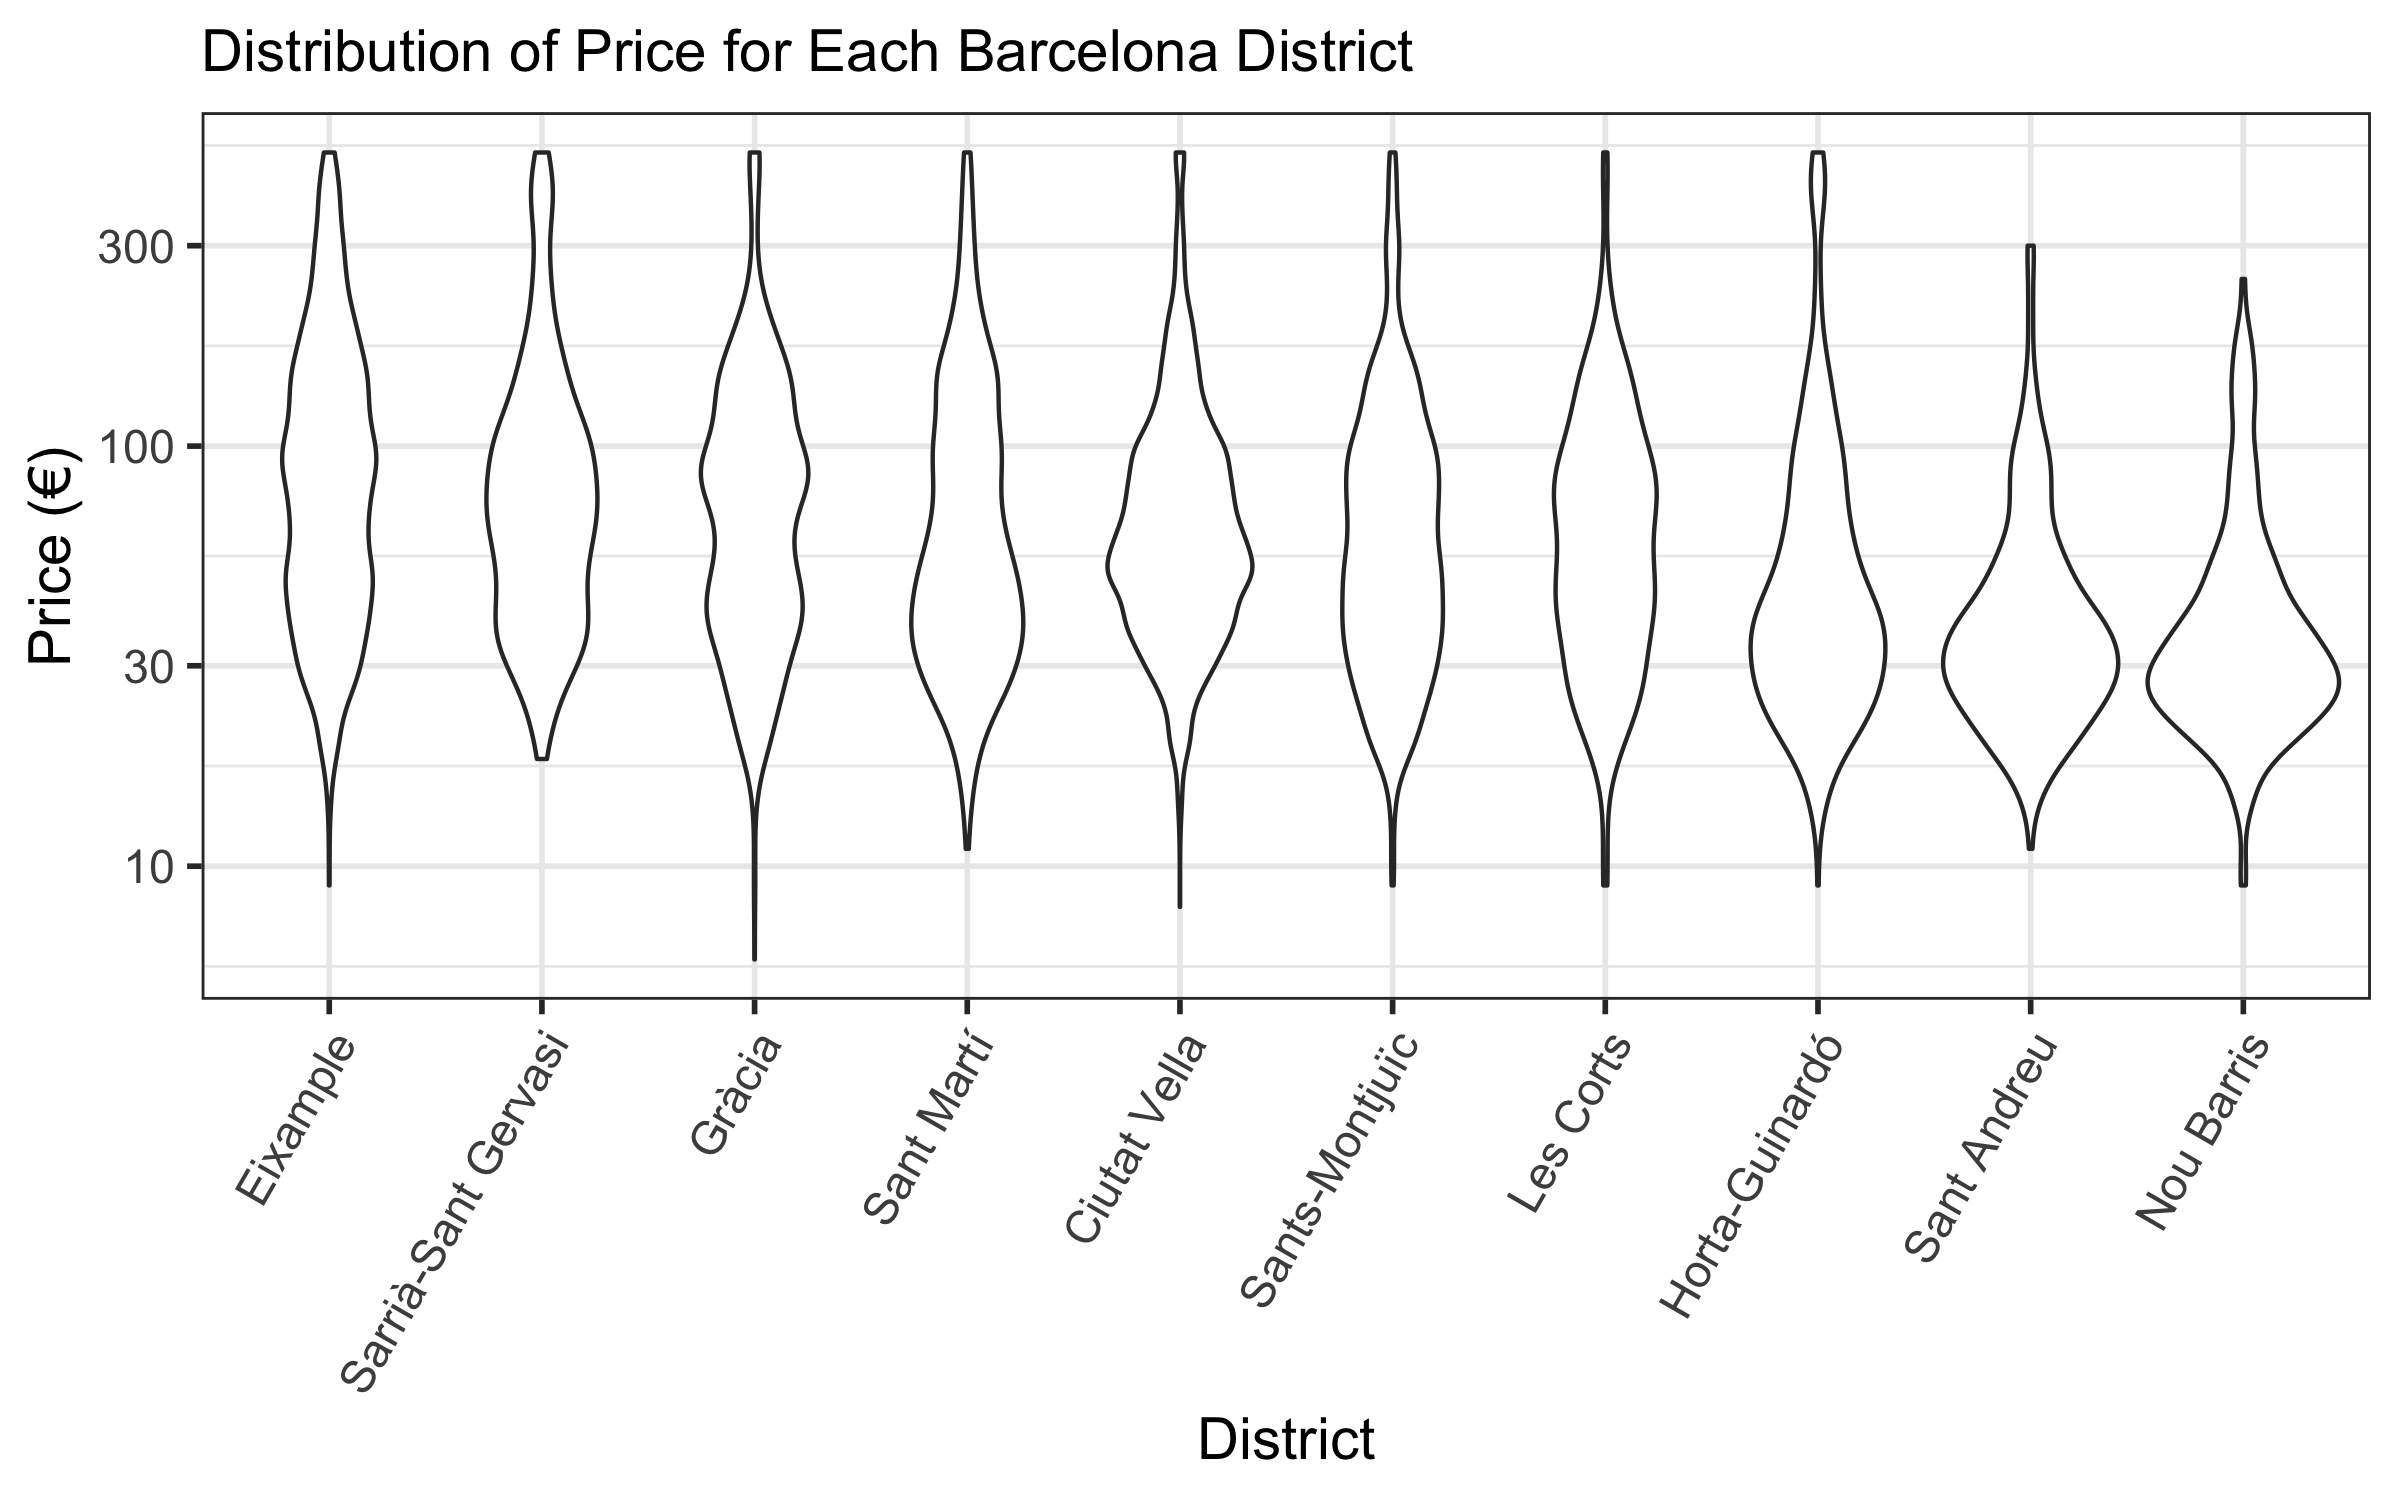
\includegraphics[width=7.03125in,height=\textheight]{../images/violin_plot.png}

\hypertarget{methods}{%
\subsubsection{Methods}\label{methods}}

We performed linear regression on Airbnb listing's of price to district,
type of room, reviews left per month, and distance from city center to
see how these variables my be affecting the Airbnb listing prices in
Barcelona. A QQ-plot was created to assess the linear model probability
residuals distributions to a normal distribution.

\hypertarget{results}{%
\subsubsection{Results}\label{results}}

We are interested in the linear relationship between an Airbnb listing's
district, type of room, reviews left per month, and distance from city
center to the listing's price. The results of the linear model are
presented below.

\begin{Shaded}
\begin{Highlighting}[]
\NormalTok{lm}\FloatTok{.1}\NormalTok{ <-}\StringTok{ }\KeywordTok{readRDS}\NormalTok{(}\DataTypeTok{file=}\NormalTok{here}\OperatorTok{::}\KeywordTok{here}\NormalTok{(}\StringTok{"data"}\NormalTok{, }\StringTok{"lm1_results.rds"}\NormalTok{))}
\NormalTok{lm}\FloatTok{.2}\NormalTok{ <-}\StringTok{ }\KeywordTok{readRDS}\NormalTok{(}\DataTypeTok{file=}\NormalTok{here}\OperatorTok{::}\KeywordTok{here}\NormalTok{(}\StringTok{"data"}\NormalTok{, }\StringTok{"lm2_results.rds"}\NormalTok{))}
\KeywordTok{tidy}\NormalTok{(lm}\FloatTok{.1}\NormalTok{)}
\end{Highlighting}
\end{Shaded}

\begin{verbatim}
## # A tibble: 15 x 5
##    term                        estimate std.error statistic  p.value
##    <chr>                          <dbl>     <dbl>     <dbl>    <dbl>
##  1 (Intercept)                  154.        1.76     87.6   0.      
##  2 districtEixample              13.7       1.84      7.44  1.05e-13
##  3 districtGràcia                -0.959     2.80     -0.342 7.32e- 1
##  4 districtHorta-Guinardó         4.49      3.92      1.14  2.53e- 1
##  5 districtLes Corts              0.938     5.09      0.184 8.54e- 1
##  6 districtNou Barris             4.50      6.08      0.741 4.59e- 1
##  7 districtSant Andreu           -3.51      5.11     -0.687 4.92e- 1
##  8 districtSant Martí             4.21      2.49      1.69  9.02e- 2
##  9 districtSants-Montjuïc        -2.76      2.67     -1.03  3.02e- 1
## 10 districtSarrià-Sant Gervasi   18.2       4.20      4.33  1.48e- 5
## 11 room_typeHotel room           30.7       3.58      8.58  1.03e-17
## 12 room_typePrivate room        -89.9       1.20    -74.7   0.      
## 13 room_typeShared room         -92.5       6.85    -13.5   3.19e-41
## 14 distance                    -489.       68.2      -7.17  7.80e-13
## 15 reviews_per_month             -3.13      0.320    -9.80  1.40e-22
\end{verbatim}

\begin{Shaded}
\begin{Highlighting}[]
\KeywordTok{tidy}\NormalTok{(lm}\FloatTok{.2}\NormalTok{)}
\end{Highlighting}
\end{Shaded}

\begin{verbatim}
## # A tibble: 15 x 5
##    term                        estimate std.error statistic   p.value
##    <chr>                          <dbl>     <dbl>     <dbl>     <dbl>
##  1 (Intercept)                   4.98     0.0137    363.    0.       
##  2 districtEixample              0.0771   0.0144      5.36  8.49e-  8
##  3 districtGràcia               -0.0280   0.0219     -1.28  2.00e-  1
##  4 districtHorta-Guinardó       -0.107    0.0306     -3.48  4.99e-  4
##  5 districtLes Corts             0.0537   0.0398      1.35  1.77e-  1
##  6 districtNou Barris           -0.0810   0.0475     -1.71  8.79e-  2
##  7 districtSant Andreu          -0.181    0.0399     -4.53  5.90e-  6
##  8 districtSant Martí           -0.0238   0.0194     -1.22  2.21e-  1
##  9 districtSants-Montjuïc       -0.0706   0.0209     -3.38  7.26e-  4
## 10 districtSarrià-Sant Gervasi   0.177    0.0328      5.39  7.11e-  8
## 11 room_typeHotel room          -0.0167   0.0280     -0.598 5.50e-  1
## 12 room_typePrivate room        -1.01     0.00940  -108.    0.       
## 13 room_typeShared room         -1.27     0.0536    -23.7   9.59e-122
## 14 distance                     -6.25     0.533     -11.7   1.28e- 31
## 15 reviews_per_month            -0.0214   0.00250    -8.57  1.18e- 17
\end{verbatim}

\begin{Shaded}
\begin{Highlighting}[]
\KeywordTok{augment}\NormalTok{(lm}\FloatTok{.1}\NormalTok{)}
\end{Highlighting}
\end{Shaded}

\begin{verbatim}
## # A tibble: 13,590 x 13
##    .rownames price district room_type distance reviews_per_mon~ .fitted .se.fit
##    <chr>     <dbl> <chr>    <chr>        <dbl>            <dbl>   <dbl>   <dbl>
##  1 1           130 Sant Ma~ Entire h~  0.0253             0.02    146.     1.92
##  2 2            60 Eixample Entire h~  0.0224             0.25    156.     1.25
##  3 3           210 Sant Ma~ Entire h~  0.0482             0.48    133.     2.36
##  4 4            32 Gràcia   Private ~  0.0312             2.38     40.2    2.01
##  5 5            60 Gràcia   Entire h~  0.0343             1.71    131.     2.02
##  6 6            70 Gràcia   Entire h~  0.0330             0.84    134.     2.03
##  7 7           140 Gràcia   Entire h~  0.0244             0.580   139.     2.09
##  8 8           100 Ciutat ~ Private ~  0.00820            0.07     59.6    1.51
##  9 9           250 Ciutat ~ Entire h~  0.00708            1.28    146.     1.55
## 10 10           40 Eixample Private ~  0.0301             2.97     53.5    1.25
## # ... with 13,580 more rows, and 5 more variables: .resid <dbl>, .hat <dbl>,
## #   .sigma <dbl>, .cooksd <dbl>, .std.resid <dbl>
\end{verbatim}

\begin{Shaded}
\begin{Highlighting}[]
\KeywordTok{glance}\NormalTok{(lm}\FloatTok{.1}\NormalTok{)}
\end{Highlighting}
\end{Shaded}

\begin{verbatim}
## # A tibble: 1 x 11
##   r.squared adj.r.squared sigma statistic p.value    df  logLik    AIC    BIC
##       <dbl>         <dbl> <dbl>     <dbl>   <dbl> <int>   <dbl>  <dbl>  <dbl>
## 1     0.360         0.359  65.3      545.       0    15 -76071. 1.52e5 1.52e5
## # ... with 2 more variables: deviance <dbl>, df.residual <int>
\end{verbatim}

The QQ-plot is presented to assess whether the assumption of normally
distributed residuals is reasonable. We can see that the residuals have
an extremely heavy upper tail and a light lower tail. This plot shows
pretty convincing evidence that the normality assumption is not
appropriate. For a better model, perhaps we should try transformations
of the variables such as a log transformation of price.

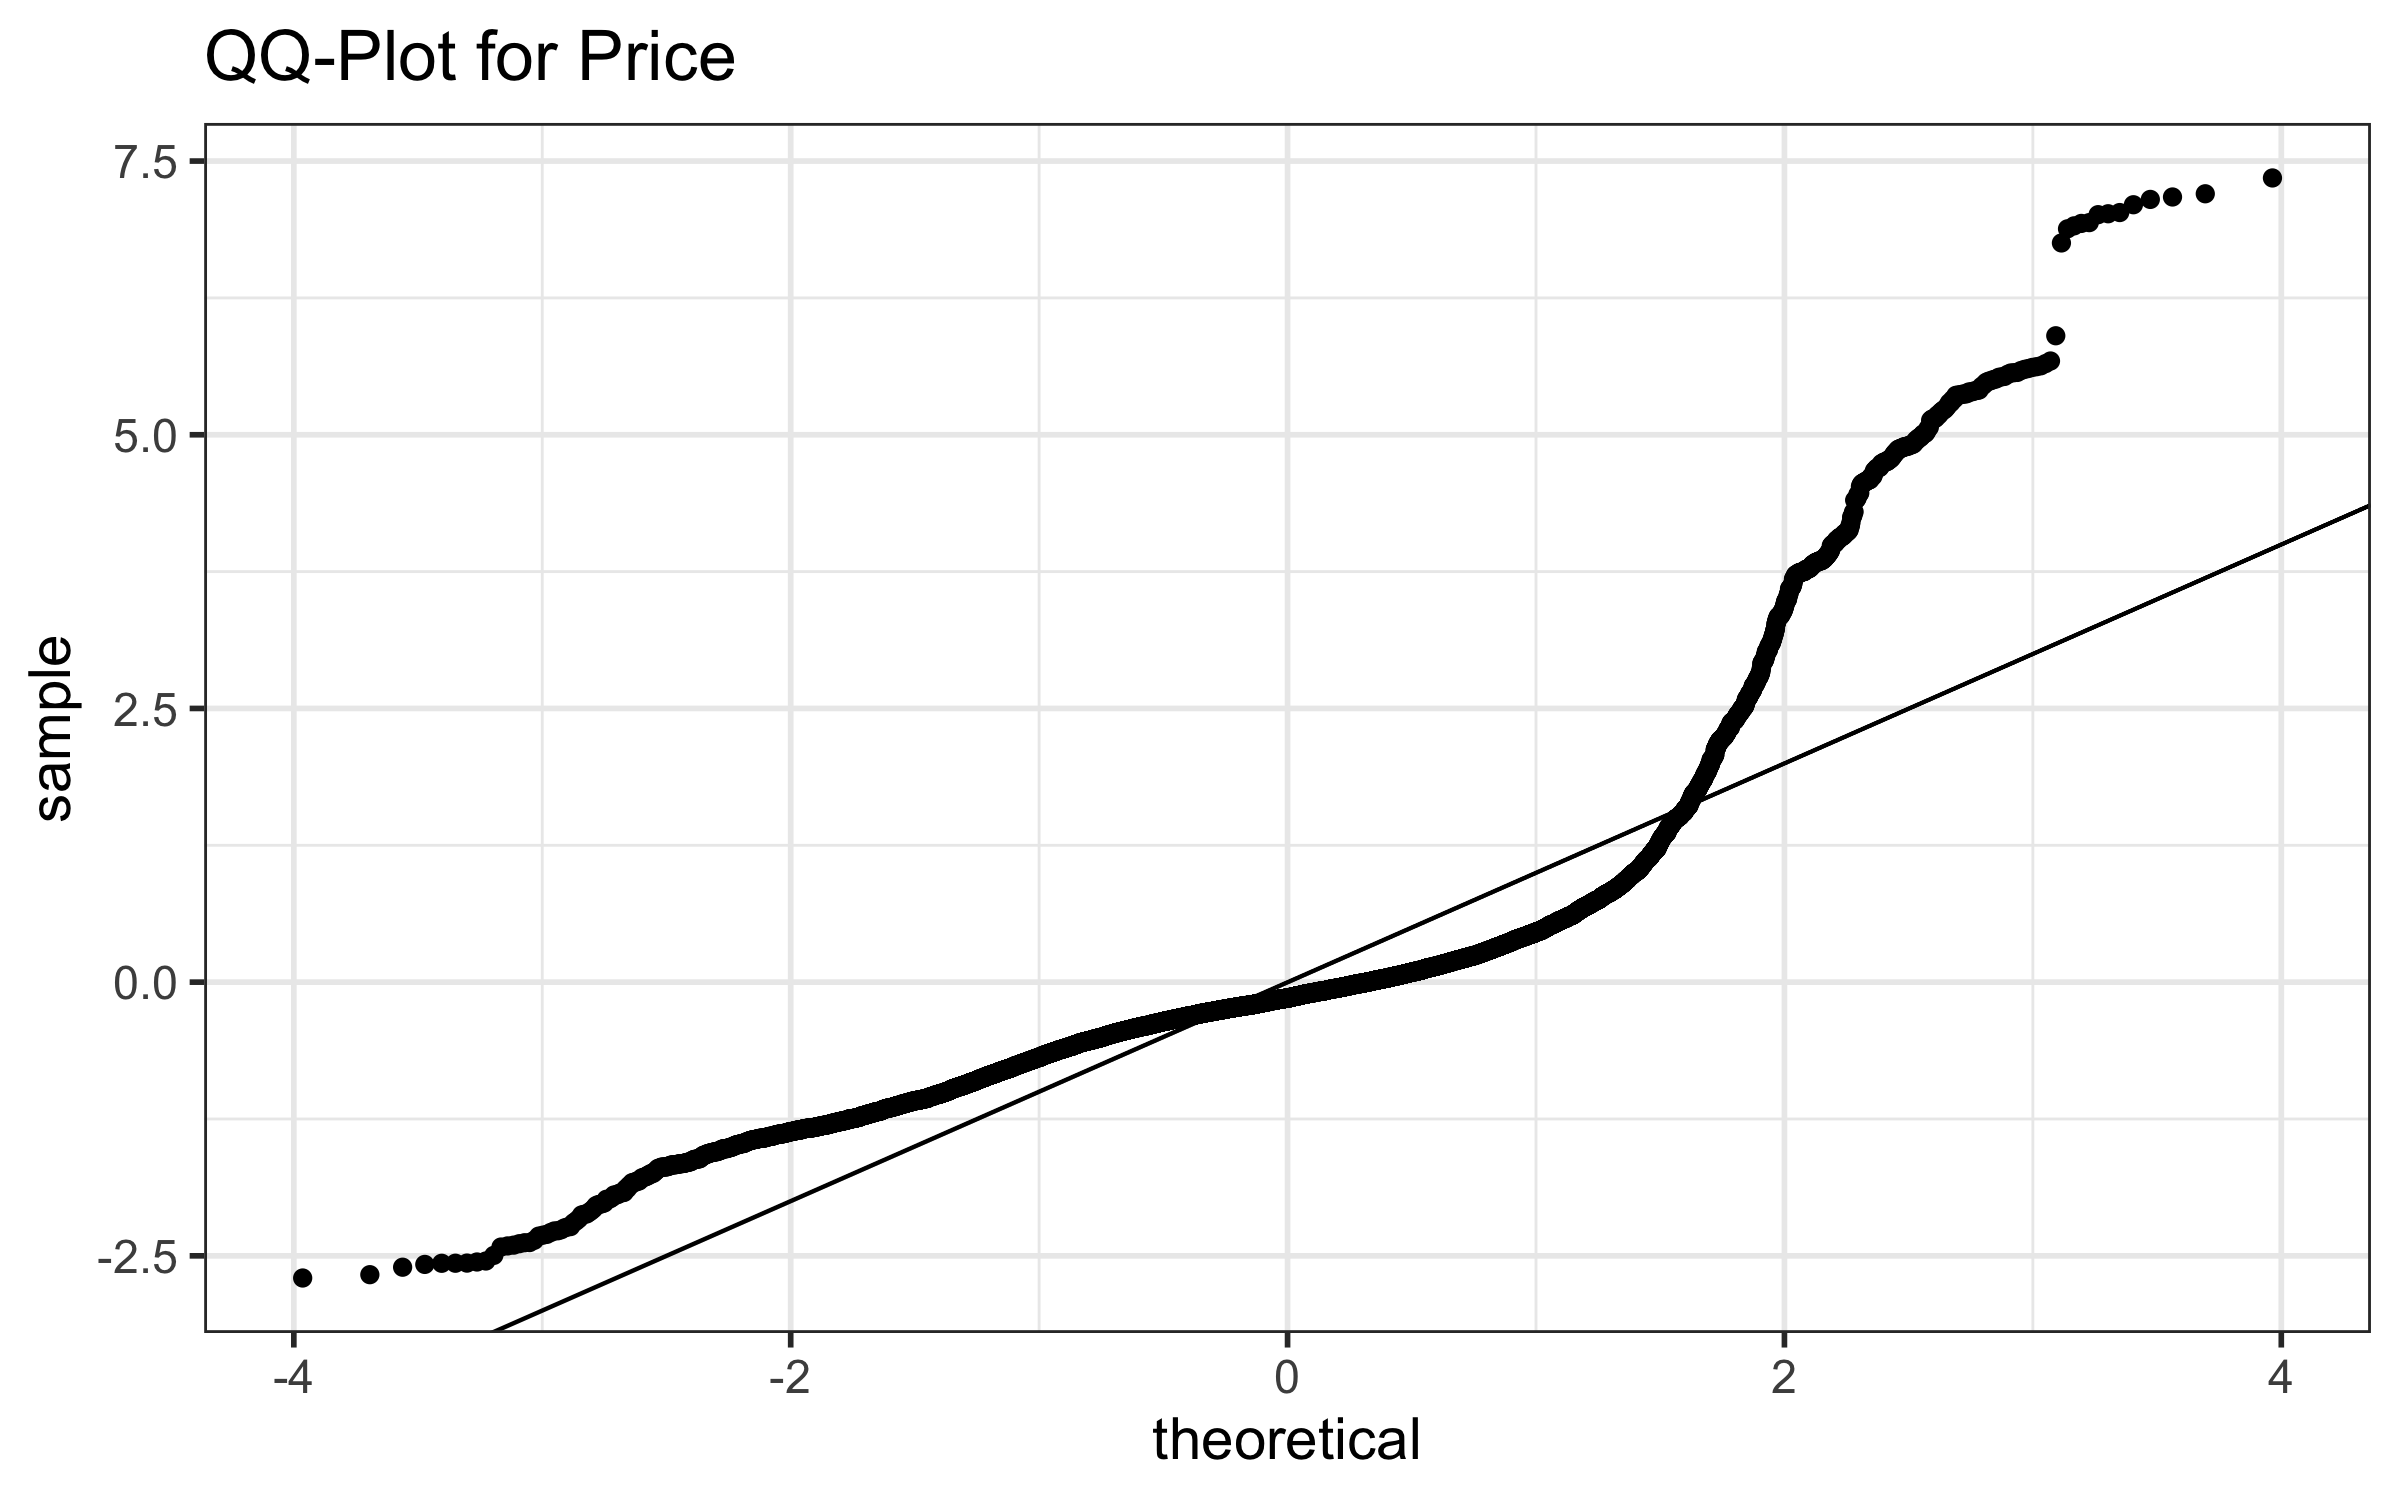
\includegraphics[width=4.6875in,height=\textheight]{../images/lm1-QQPlot.png}
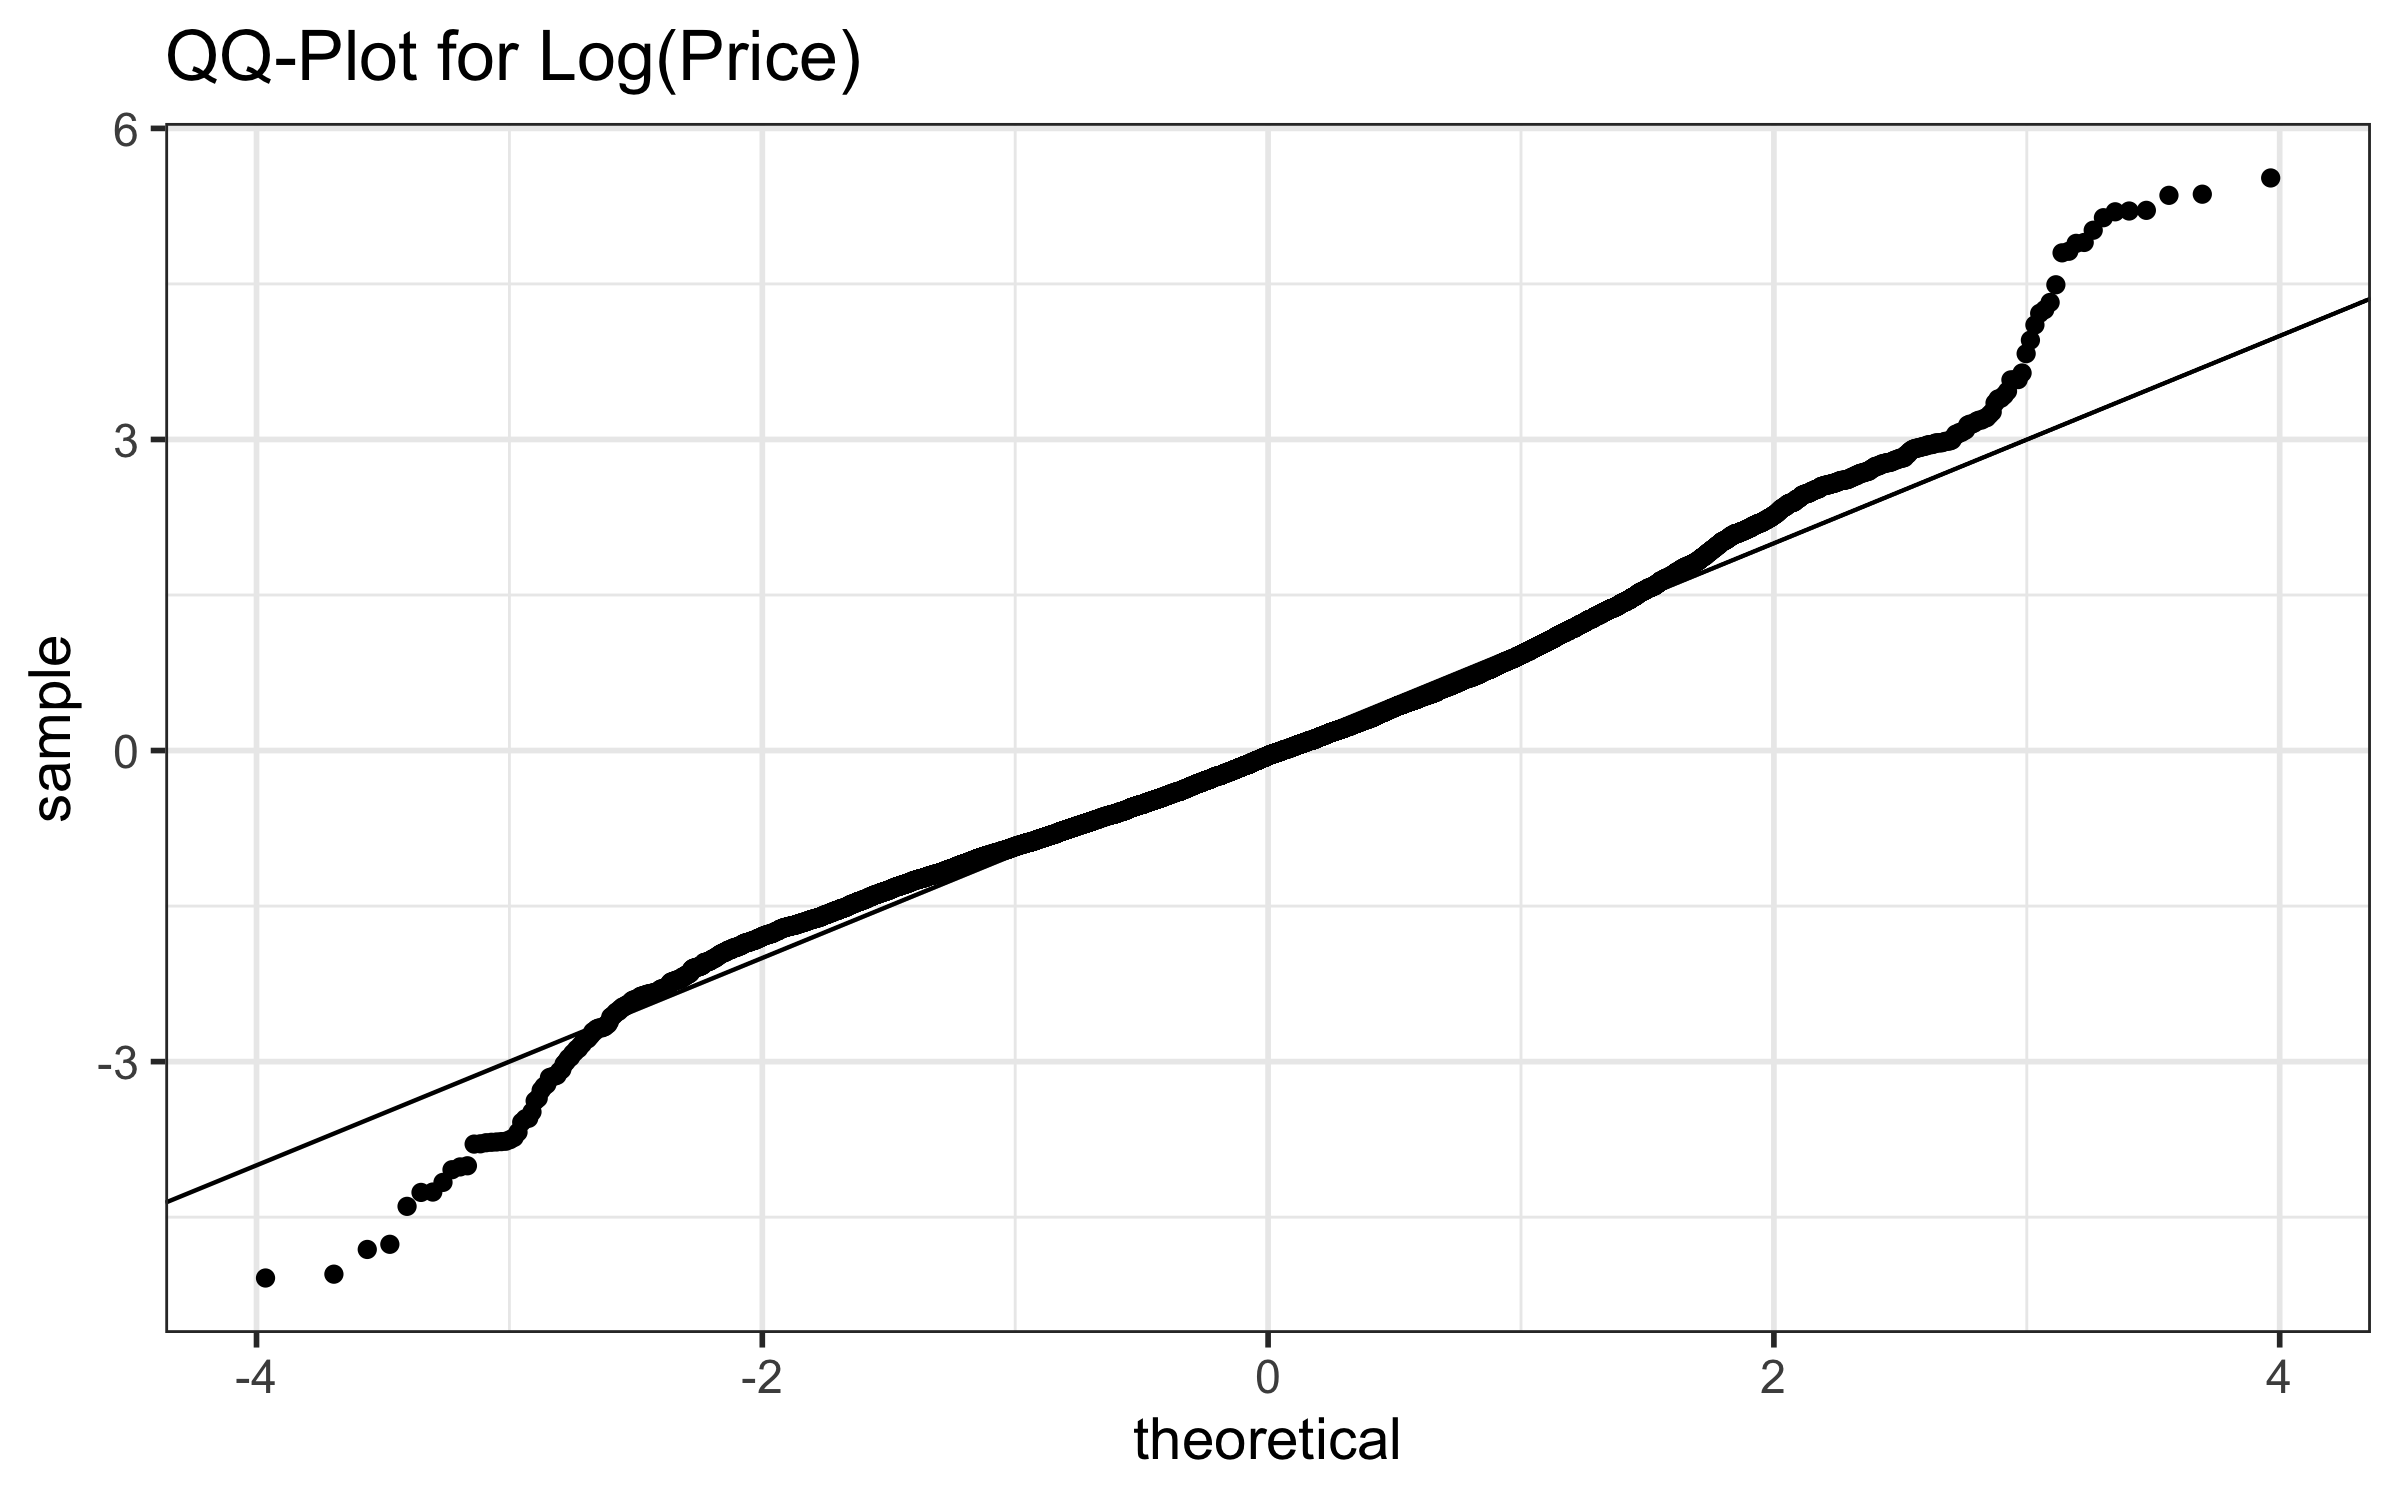
\includegraphics[width=4.6875in,height=\textheight]{../images/lm2-QQPlot.png}

\hypertarget{discussion}{%
\subsubsection{Discussion}\label{discussion}}

In determining the linear relationship between an Airbnb listing's
district, type of room, reviews left per month, and distance from city
center to the listing's price, the model made has an assumption of
normal distribution. However, Based on the QQ-plot, the residuals do not
follow the linear trend and, therefore, the assumtion of a normal
distribution does not hold.

\hypertarget{references}{%
\subsubsection{References}\label{references}}

\href{http://insideairbnb.com/get-the-data.html}{Airbnb dataset}

\end{document}
